\input{../header}

\begin{document}
%


%\onehalfspacing
\allowdisplaybreaks
%##################################################################
\section{PS\#14 - The normal distribution! -- {\color{red} KEY} }

\everymath{\displaystyle}
The well-known 68-95-99.7 rule states that approximately 68\% of values of a normally-distributed random variable lie within one standard deviation of the mean. In this extended problem, we will use Taylor series to calculate this percentage directly.

Here is the equation for the ``normal probability density function'' with mean $\mu=0$ and standard deviation $\sigma=1$: \[p(x) = \frac{1}{\sqrt{2\pi}} \exp\left(\frac{-x^2}{2}\right).\]

You may know this function better by another name: the bell curve!


Throughout this problem set, when you are asked to write down a Taylor series for some function, you may either use $\Sigma$ notation or write out the first few terms of the series.
\begin{enumerate}[leftmargin=0pt]
    \item Draw a graph of $p(x)$. You can use Desmos but in a minute I'm going to ask you to shade something in so you may want something you can draw on.
    \item We want to find the proportion of values that lie within one standard deviation ($\sigma = 1$) of the mean ($\mu=0$); in other words, we want to find the proportion of values that lie less than 1 distance away from 0 in either direction. Shade in this region on your graph.
    \begin{center}
        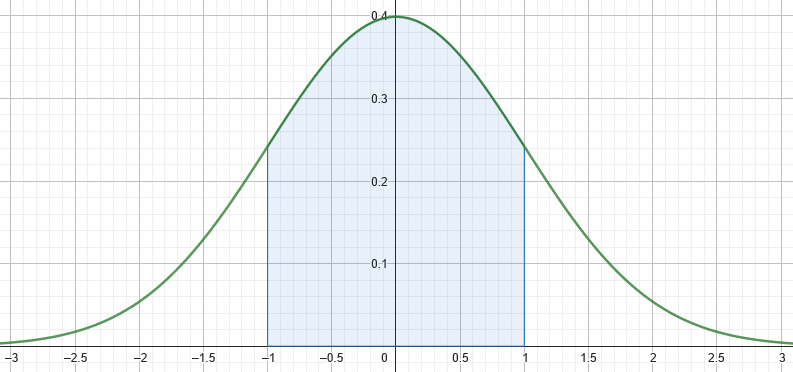
\includegraphics[width=0.8\textwidth]{../images/normal-curve-shaded.png}
    \end{center}
    
    \item We can compute this value by finding $\int_a^b p(x)\ dx$. What should our bounds of integration $a$ and $b$ be, and why?

    \begin{red}
        The bounds of integration should be from $a=-1$ to $b=1$. We want to go 1 distance away from 0 in either direction.
    \end{red}
    \item If we start by finding an antiderivative, $P(x)$, then our answer will be $P(b) - P(a)$. But unfortunately, we can't immediately write down an antiderivative $P(x)$. Why not?

    \begin{red}
        This is one of our rude functions that doesn't have an antiderivative -- the $x^2$ inside the $\exp(\ldots)$ means that substitution won't work, in particular.
    \end{red}
    \item Write down the Taylor series for $f(u) = e^u$.
    
    \begin{red}
    \[e^u = \sum_{k=0}^\infty \frac{1}{k!} u^k = 1 + \frac{u}{1!} + \frac{u^2}{2!} + \frac{u^3}{3!} + \ldots \]
    \end{red}
    \item Use the Taylor series for $e^u$ to write down the Taylor series for $p(x).$ \\ (Don't forget the $\tfrac{1}{\sqrt{2\pi}}$!)
    
    \begin{red}
    We are going to substitute $-\frac{x^2}{2}$ for all the $u$'s in the previous result, then multiply by $\frac{1}{\sqrt{2\pi}}$:
    \[p(x) = \frac{1}{\sqrt{2\pi}} \exp\left(\frac{-x^2}{2}\right) = \frac{1}{\sqrt{2\pi}} \sum_{k=0}^\infty \frac{1}{k!} \left(\frac{-x^2}{2}\right)^k = \frac{1}{\sqrt{2\pi}}\cdot \left(1 + \frac{(-x^2 / 2)}{1!} + \frac{(-x^2 / 2)^2}{2!} + \frac{(-x^2/2)^3}{3!} + \ldots \right)\]
    Simplifying a little:
    \[ p(x) = \frac{1}{\sqrt{2\pi}} \sum_{k=0}^\infty \frac{(-1)^k x^{2k}}{k!\cdot 2^k} = \frac{1}{\sqrt{2\pi}} \left(1 - \frac{x^2}{1! \cdot 2} + \frac{x^4}{2!\cdot 4} - \frac{x^6}{3!\cdot 8} + \frac{x^8}{4! \cdot 16} \ldots \right) \]
    \end{red}
    \item Use the Taylor series for $p(x)$ to write down a Taylor series for its antiderivative $P(x)$.
    
    \begin{red}
    I'm going to integrate the thing inside the sum with respect to $x$, then stick it all back in the sum. Notice that I don't need a $+C$ because this will eventually become a definite integral.
    \[\int \frac{(-1)^k x^{2k}}{k!\cdot 2^k}\ dx
    = \frac{(-1)^k }{k!\cdot 2^k} \int x^{2k} \ dx 
    = \frac{(-1)^k }{k!\cdot 2^k} \cdot \frac{x^{2k+1}}{2k+1}
    \]
    
    \[P(x) = \frac{1}{\sqrt{2\pi}} \sum_{k=0}^\infty \frac{(-1)^k x^{2k+1} }{k!\cdot 2^k \cdot (2k+1)} = \frac{1}{\sqrt{2\pi}} \left(x - \frac{x^3}{1! \cdot 2\cdot 3} + \frac{x^5}{2!\cdot 4\cdot 5} - \frac{x^7}{3!\cdot 8 \cdot 7} + \frac{x^9}{4! \cdot 16\cdot 9} \ldots \right)\]
    \end{red}
    \item Use the first four nonzero terms of the Taylor series for $P(x)$ to approximate $P(b)$. \\
    (Hint: This is probably \textit{not} the fourth-degree polynomial.)
    
    \begin{red}
    So we're going to plug $b$, which is $1$, in for $x$ in each of the first four terms of our series (the ones that come from $k=0, 1, 2, 3$):
    
    \[P(1) \approx \frac{1}{\sqrt{2\pi}} \left(1 - \frac{1^3}{1! \cdot 2\cdot 3} + \frac{1^5}{2!\cdot 4\cdot 5} - \frac{1^7}{3!\cdot 8 \cdot 7}\right)\]
    
    According to Wolfram Alpha, that's $\frac{1}{\sqrt{2\pi}}\cdot  \frac{479}{560} \approx 0.34124$.
    
    (Notice, btw, that this is indeed \textit{not} the fourth-degree polynomial -- it's the 7th-degree polynomial. This is actually good because higher powers of $x$ are probably going to give us better approximations, so it's nice when they come earlier in the series than we would otherwise think.)
    \end{red}
    \item Use the first four nonzero terms of the Taylor series for $P(x)$ to approximate $P(a)$. \\
    (Hint: This is probably \textit{not} the fourth-degree polynomial.)
    
    \begin{red}
    Similar: we're going to plug $a$, which is $-1$, in for $x$ in each of the first four terms of our series:
    \[P(-1) \approx \frac{1}{\sqrt{2\pi}} \left((-1) - \frac{(-1)^3}{1! \cdot 2\cdot 3} + \frac{(-1)^5}{2!\cdot 4\cdot 5} - \frac{(-1)^7}{3!\cdot 8 \cdot 7} \right) = \frac{1}{\sqrt{2\pi}} \left(-1 + \frac{1^3}{1! \cdot 2\cdot 3} - \frac{1^5}{2!\cdot 4\cdot 5} + \frac{1^7}{3!\cdot 8 \cdot 7}\right) \]
    
    According to Wolfram Alpha, that's $-\frac{1}{\sqrt{2\pi}}\cdot  \frac{479}{560} \approx -0.34124$.
    \end{red}
    \item Find $P(b) - P(a)$. (Your answer should be close to 68\%.)
    
    \begin{red}
    \[P(1) - P(-1) \approx \frac{1}{\sqrt{2\pi}}\cdot  \frac{479}{560} - \left( - \frac{1}{\sqrt{2\pi}}\cdot  \frac{479}{560}\right) \approx 0.34124 + 0.34124 = 0.68248.\]
    \end{red}
    \item How many terms would be necessary to ensure that your approximation to $P(b)-P(a)$ is accurate to four decimal places? 
    
    \begin{red}
    We're going to use the alternating series error bound:
    \[\text{If } S = \sum_{k=0}^\infty (-1)^k a_k\text {, then }|S-S_n| < |a_{n+1}|.\]
    That is, the ``truncation error'' that's produced by using a partial sum to approximate the full sum is bounded by the size of the next term.

    A tricky thing here is that we are actually using \textit{two} values, so we get a little bit of error from both ends of our calculation. Conveniently, $P(-1) = -P(1)$, so $P(1) - P(-1) = 2P(1)$. Therefore we can figure out the error for just $P(1)$ and then \textit{double} it.
    
    Since our Taylor series is alternating, we just need to look at the size of each term:
    \[|a_k| = \left|\frac{1}{\sqrt{2\pi}} \cdot \frac{(-1)^k \cdot x^{2k+1} }{k!\cdot 2^k\cdot(2k+1)} \right| = \frac{1}{\sqrt{2\pi}} \cdot \frac{1}{k!\cdot 2^k\cdot(2k+1)}\] and determine when they start being less than $5\times 10^{-5}$. Here is a table of values -- note that I have already doubled them.
    \[
\begin{array}{c|c|c|c|c|c|c}
k     & 1         & 2         & 3         & 4         & 5         & 6         \\\hline
|a_k| & 0.1329808 & 0.0199471 & 0.0023747 & 0.0002309 & 0.0000189 & 0.0000013
\end{array}
    \]
    So the first term that's smaller than $5\times10^{-5}$ is $|a_5|$, which means we need $k=4$, which means we need five terms. (Remember, $k$ starts counting at 0.)

    You can check that our five-term approximation is about $0.6827071$ -- so we can be confident that the true value rounded to the fourth decimal place is exactly $0.6827$.
    
    (Aside: The Lagrange error bound is probably a bad idea here because the pattern in the derivatives is, uh, \href{https://math.stackexchange.com/questions/1488210/how-to-get-nth-derivative-of-ex2-2}{complicated}.)
    \end{red}
\end{enumerate}
\end{document}